\documentclass{task_description}

\usepackage{xcolor}
\usepackage{pdfpages} 
\newcommand\notes[1]{\textcolor{red}{#1}}

\begin{document}

\thispagestyle{firstpage}
\vspace*{23mm}%
\hfill\parbox[t]{65mm}{

Timothy Zemp\\
Hagenholzstrasse 92\\
8052 Z\"urich\\[5mm]
Matrikel-Nr. 13-915-632\\
timothy.zemp@uzh.ch\\[15mm]
%\today
July 24, 2020 \\
}
\vspace*{5mm}
\subsection*{Master's Thesis Specification}
%
%\section*{Title:\\  "Supporting Developers during Unit and Integration Testing by improving the TestDescriber Tool"\hspace{1em}}
\section*{Separating wheat from chaff: Detecting genuine Continuous Integration configurations\hspace{1em}}

Continuous Integration (CI) is a software development practice introduced by the Agile movement with the aim of delivering reliable software releases fastly \cite{Humble:2010}. Whenever a change is pushed in a remote software repository (\eg GitHub), a build server tool (\eg Travis-CI) detects this change and triggers the integration pipeline. The pipeline typically consists of several steps \eg compilation, unit testing, packaging, integration testing, installation and deploy and is usually defined within a configuration file (\eg .travis-ci.yml).

CI has also been an uprising topic in empirical research, studying the impact of CI on code review or developer's behaviour. Notable studies showed that for example CI leads to a higher code commitment frequency and reduced code chunks \cite{zhao2017impact}, different programming languages showes different adoption times (\eg Ruby as being an early-adopter, whereas Java projects tend to adopt later)\cite{vasilescu2014continuous}, and proper build configurations should be maintained in order to reduce long build durations\cite{ghaleb2019empirical}.
Cloud CI providers (\eg Travis-CI, Jenkins) are easy to adopt and once a repository is registered, it is sufficient to commit a configuration file into the repository. Due to this simple process, many public repositories contain such configuration files, but naturally, many of them do not use CI seriously. Unfortunately, many studies do not differentiate and typically treat every project with a configuration file as a valid instance (\eg \cite{zhao2017impact}, \cite{vasilescu2014continuous}, \cite{ghaleb2019empirical}), which might dilute the results. 

Inspired by the work of Munaiah et al.\cite{munaiah2017curating}, where they implemented and validated a tool (reaper\footnote{https://github.com/RepoReapers/reaper}) to asses the quality of a GitHub repository, we aim to lower the tread to validity of empirical studies on CI by providing a classifier which evaluate the \textit{genuineness} of pipeline configurations. Reaper provides a score which assesses the likelihood of the repository containing engineered software separating it from potential noise (\eg home work assignments, study projects, ...). The tool works by identifying different practices, called dimensions (\eg documentation, testing, history, ...) and classify them using both a Score-Based Classifier as well as a Random Forst Classifier. By establishing a Ground Truth Dataset and extracting features on the pipeline configuration, we aim to assess the quality of CI within a software repository.

\subsection*{The goals of this Master's thesis}

The goal of this master's thesis is to identify genuine configurations that qualitative CI typically express with the intention to generalize those in order to identify software repositories or configuration adopting these practices. Such a classifier (similar to reaper) would either accepts an CI configuration file or a software repository and outputs a score on the quality of the CI within the software repository. This will allow future studies to filter out software projects that do not have genuine CI configurations, picking only those who uses CI at a high level of quality.
\\\\
Whilst developing the classifier, the following research questions arise:
\\\\
\textbf{RQ 1: Why does software projects have pseudo configuration files?}\\
First we analyze why software projects might have pseudo configurations (\ie in opposite to genuine configurations). This will enable us to extract features of genuine CI configurations.
\\\\
\textbf{RQ 2: What is the accuracy (Precision \& Recall) of an automated detection of meaningful CI configurations?}\\
In RQ 2 we focus on measuring the accuracy of our classifier. By segment-comparing (approx. 10\%) of our manually labeled reference-set we calculate precision (false positive rate) and recall (false negative rate) and hence measure the accuracy of the classifier.
\\\\
\textbf{RQ 3: Are features extract only from the configuration sufficient to classify accurately or is a more broader context required?}\\
The features of our classifier can be grouped into three categories, each representing a different level (\ie higher \& more difficult) on how those features are obtained: \textit{configuration-level}, \textit{repository-level} and \textit{pipeline-level}. In RQ 3 we analyze whether the lowest level of access (configuration-level) is sufficient to yield accurate classifications, or more broader features (repository-level or pipeline-level) are required.
\\\\
\textbf{RQ 4: Does the classification obtained by \textit{reaper} correlate with our classification?}\\
RQ 4 aims to reveal whether there is a correlation between engineered software projects, classified by \textit{reaper} and software repositories having a genuine CI configuration (classified by our classifier).
\\\\
\textbf{RQ 5: What impact does the classifier has on CI-based studies?}\\
In the last research question we want to asses the impact of the classifier to already existing empirical CI-studies. Using a large-scale dataset we aim to reproduce previous studies where one for example has analyzed the impact of the programming language towards the adoption of CI, or the impact of CI on the software's quality, but applying our classifier to the selection of the analyzed projects. 
\newpage
\subsection*{Task description}

The main tasks of this thesis are:
\\\\
\bgroup
\def\arraystretch{1.1}%  1 is the default, change whatever you need
\begin{tabular}{lp{10cm}}  
 ID & Task \\
\hline\noalign{\smallskip}
 T1 & Research on the topic of CI and the different pipeline configuration mechanism \\
 T2 & Data Collection of various repositories using CI and labeling them to establish Ground truth \\
 T3 & Definition of extracted features (RQ 1)\\
 T4 & Development of classifier\\
 T5 & Evaluate the classifier using the reference set and statistical methods (RQ 2/3)\\
 T6 & Evaluate correlation between \textit{repaer} and the classifier (RQ 4)\\
 T7 & Identify existing CI-studies and evaluate the impact of the classifier (RQ 5)\\
 T8 & Write a thesis, comprising the points above\\
\hline
\end{tabular}
\egroup

\subsection*{Thesis Structure \& Deliverable}

The thesis consists of several parts. First, basic research is required in order to gain an overview of the different pipeline providers and the possibilities of CI. Afterwards, a Ground Truth Dataset (D1) is established by collecting various repositories adopting CI and labelling them accordingly. Using the data set, suitable features will be identified (RQ 1) and implemented in the classifier. Once enough features are implemented, the classifier is implemented using a prediction algorithm. We conclude the implementation by wrapping the classifier with a Docker Container (D2). This allows other research to easy use the classifier and reproduce our work. We then evaluate the classifier internally (RQ 2/3), evaluate the correlation towards \textit{reaper} (RQ 4) and finally observe the impact of the classifier on existing empirical CI-based studies (RQ 5). Lastly, the thesis is concluded with an academic report.
\\\\
A detailed project plan including the milestones is attached to this proposal and can be found on page \pageref{gantt}.
\\\\
\begin{tabular}{lp{10cm}}  
 ID & Deliverable \\
\hline\noalign{\smallskip}
 D1 & Ground Truth Dataset \\
 D2 & Classifier \\
 D3 & Thesis\\
\hline
\end{tabular}

\subsection*{Provided resources}

The student does not need any specific resources other than the starting literature, which is referenced in this document. A workplace in the s.e.a.l. lab will be at disposal.

\newpage
\subsection*{General thesis guidelines}

The typical rules of academic work must be followed. In Bernstein \cite{Bernstein:8} describes a number of guidelines which must be followed. At the end of the thesis, a final report has to be written. The report should clearly be organized, following the usual academic report structure, and has to be written in English using our s.e.a.l. \LaTeX-template. As implementing software is also part of this thesis, State-of-the-Art
design, coding, and documentation standards for the software have to be obeyed. The product of the thesis is the Ground Truth Dataset, a working classifier as well as the written report, that summarizes the process of developing the tool and its evaluation.

\subsection*{Advisors:}

\noindent\textbf{Professor}: \\
\noindent Prof. Dr. Harald C. Gall \\
\\
\noindent\textbf{Responsible assistants}: \\
\noindent Dr.-Ing. Sebastian Proksch (TU Delft) \\


\vspace{2em}
\noindent\textbf{Signatures:}

\vspace{3\baselineskip}
\noindent Timothy Zemp\hfill Prof. Dr. Harald C. Gall
\clearpage
\label{gantt}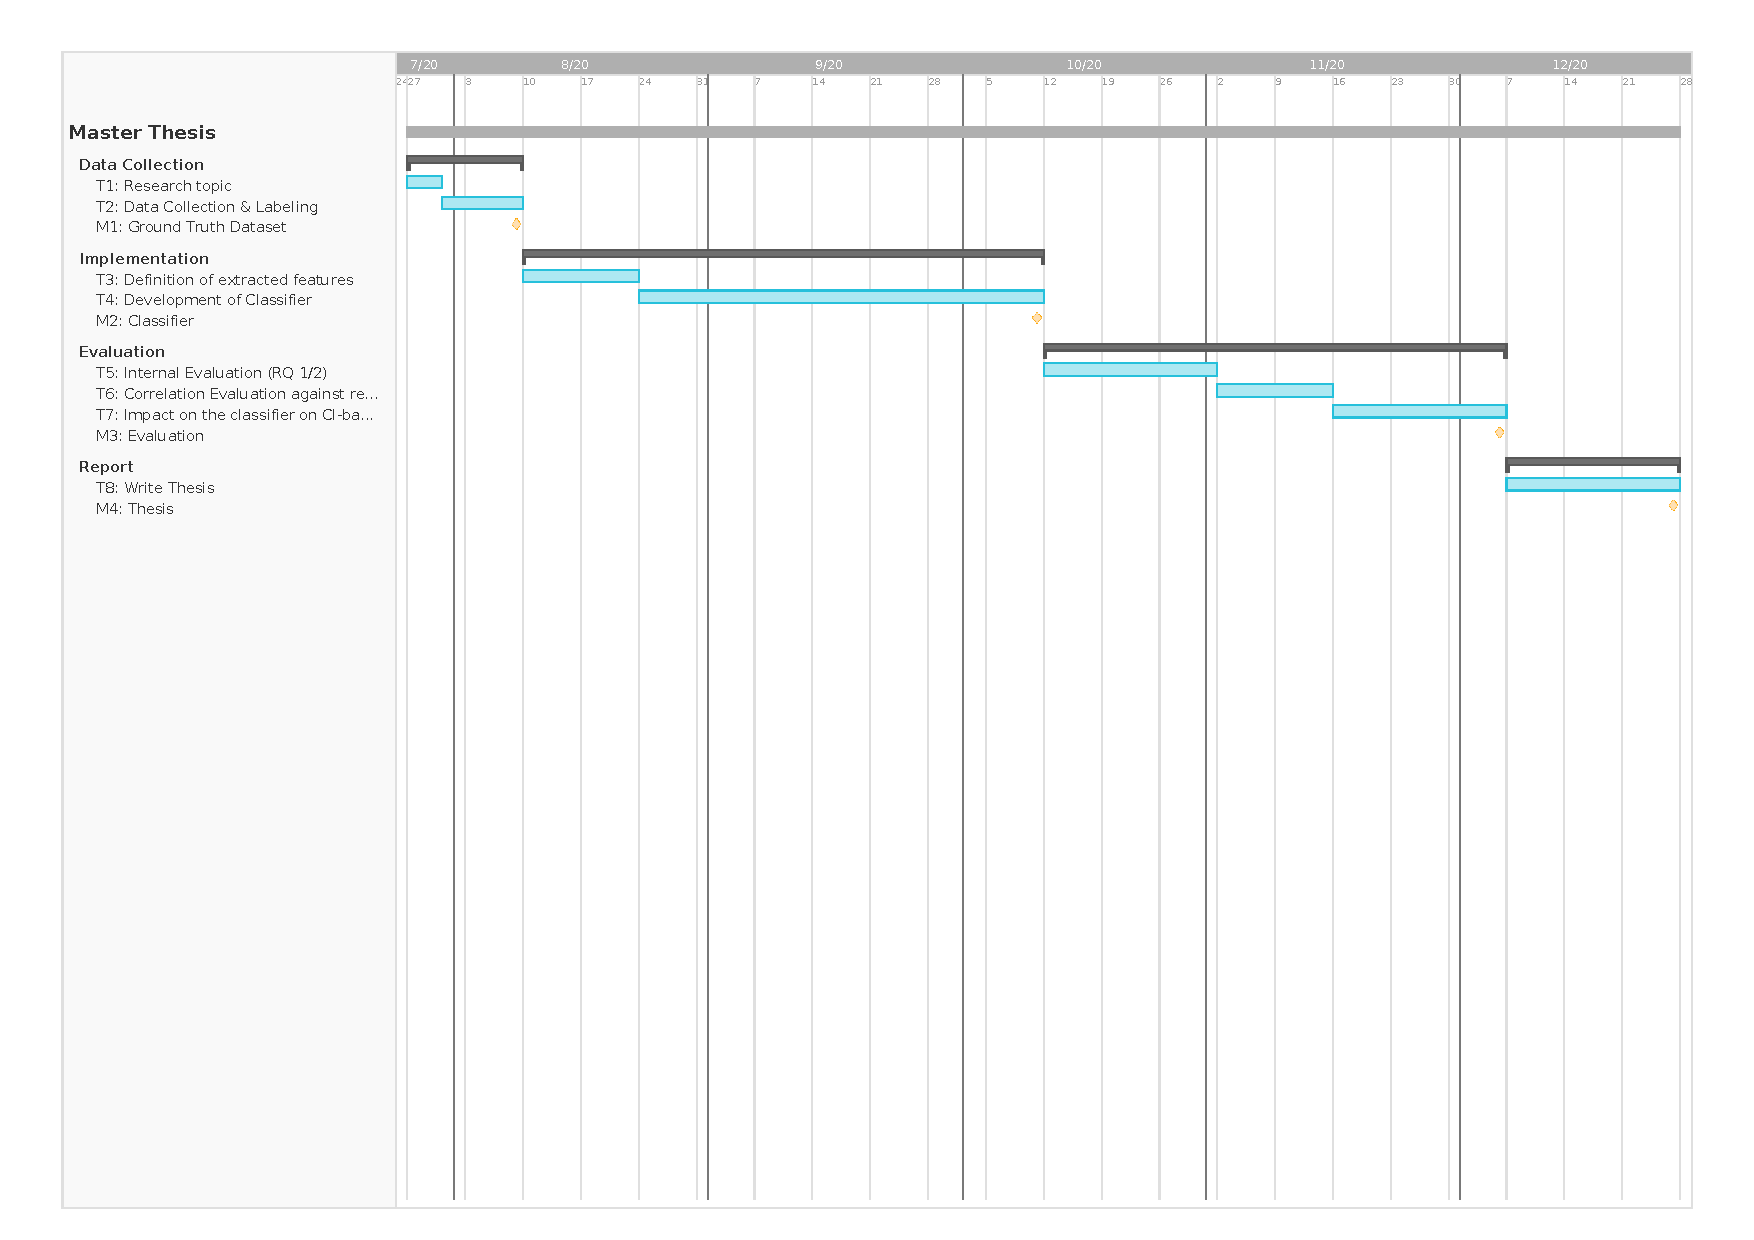
\includepdf[pages={-},fitpaper,rotateoversize]{gantt.pdf}
\bibliographystyle{abbrv}
\bibliography{refs}

\end{document}
